\capitulo{3}{Conceptos teóricos}

En este apartado se exponen los principales conceptos teóricos necesarios para comprender el funcionamiento y objetivos del proyecto \textit{Asistente de prácticas ágiles para repositorios en GitHub}, desde los fundamentos del control de versiones y GitHub, hasta las prácticas ágiles y métricas de calidad en el desarrollo software.

\section{Repositorios de GitHub}

GitHub es una plataforma de desarrollo colaborativo basada en Git que añade funcionalidades adicionales orientadas a la gestión de proyectos, la colaboración remota y la revisión de código. GitHub proporciona una interfaz web amigable que facilita la visualización del historial, la discusión de cambios, el control de versiones del repositorio y la organización del trabajo en equipo. Entre sus funcionalidades clave destacan:

\begin{itemize}
\item Repositorios y ramas: Permiten organizar el código en estructuras jerárquicas y paralelas. Las ramas facilitan el desarrollo simultáneo de nuevas funcionalidades o corrección de errores sin interferir con el código principal.
\item \textit{Issues}: Herramienta integrada para el seguimiento de tareas, errores y solicitudes de mejora. Facilitan la comunicación entre los miembros del equipo y permiten priorizar el trabajo pendiente.
\item \textit{Pull requests}: Mecanismo para proponer y discutir cambios antes de su integración en la rama principal. Incluyen herramientas de revisión de código y validación automática mediante tests o \textit{workflows}.
\item \textit{releases}: Etiquetas versionadas que marcan hitos importantes del software, como entregas estables o versiones beta. Permiten identificar fácilmente el estado de madurez del proyecto.
\item Estadísticas y métricas de calidad de proceso: GitHub ofrece paneles con datos sobre actividad reciente, contribuciones individuales, frecuencia de \textit{commits}, entre otros indicadores clave del desarrollo del proyecto.
\end{itemize}

El análisis automático de estas métricas y datos permite extraer información objetiva sobre la calidad, salud y evolución de un proyecto de software. Esto es especialmente útil para evaluar repositorios de forma sistemática, identificar buenas prácticas o detectar áreas que requieren atención.

\section{Métricas del proceso de desarrollo de repositorios}
Evaluar la calidad de un repositorio de software no solo implica revisar el código, sino también analizar cómo se gestiona y se desarrolla el proyecto en su conjunto. Esta última evaluación es la que desarrolla este proyecto empleando las prácticas ágiles. Para ello, se definen métricas cuantitativas derivadas de la actividad registrada en el repositorio, que permiten realizar una evaluación objetiva y reproducible. Algunas de las métricas más relevantes incluyen:

\begin{itemize}
\item Número medio de \textit{commits}: Indica la frecuencia con la que se realizan cambios en el código. Una actividad constante sugiere un proyecto en desarrollo activo, mientras que largos periodos sin \textit{commits} pueden señalar abandono o pausas.
\item Tiempo medio de cierre de \textit{issues}: Mide la eficiencia en la resolución de tareas o problemas. Tiempos de respuesta cortos suelen estar asociados a una buena organización y seguimiento, mientras que los retrasos pueden indicar falta de recursos o planificación.
\item Frecuencia de publicación de \textit{releases}: Refleja el ritmo de entregas del proyecto. Una cadencia regular sugiere una metodología estructurada, como la entrega incremental propia de metodologías ágiles.
\end{itemize}

Estas métricas permiten identificar patrones de trabajo, detectar cuellos de botella y sugerir mejoras conforme a las buenas prácticas del desarrollo ágil y colaborativo. Además, se pueden utilizar para monitorizar detalladamente la evolución de un mismo proyecto a lo largo del tiempo.

\section{Prácticas ágiles}
Las prácticas ágiles representan un conjunto de principios y prácticas orientadas al desarrollo de software de manera iterativa, incremental y centrada en la colaboración continua entre los miembros del equipo y con los clientes. Frente a los modelos tradicionales, como el ciclo en cascada, las prácticas ágiles fomentan la adaptabilidad, la retroalimentación constante y la entrega temprana de valor.

Dentro del universo ágil destacan marcos de trabajo como Scrum o Extreme Programming (XP) \cite{beck2004extreme}, que han sido adoptados ampliamente en la industria. Estos marcos establecen roles, eventos y artefactos que ayudan a estructurar el trabajo y mejorar la comunicación del equipo. En este proyecto, se siguen principios inspirados en la guía \cite{agileSubwayMap}, la cual agrupa diversas prácticas ágiles aplicables al desarrollo de software. Entre las más relevantes se encuentran:

\begin{itemize}
\item Iteraciones y retrospectivas: Ciclos de trabajo cortos y repetitivos (sprints) al final de los cuales se evalúa lo realizado y se planifican mejoras para el siguiente ciclo.
\item Historias de usuario y definición de “Hecho”: Las historias de usuario representan funcionalidades desde el punto de vista del usuario. La definición de “Hecho” asegura que todo el equipo tiene un criterio común sobre cuándo una tarea está completada.
\item Integración continua y revisión de código: Prácticas técnicas que permiten detectar errores tempranamente, asegurar la calidad del código y facilitar la colaboración mediante herramientas automatizadas y revisiones cruzadas entre desarrolladores.
\item Visibilidad del trabajo en curso: Uso de herramientas como tableros \textit{Kanban}, \textit{issues} o sistemas de gestión de tareas para proporcionar una visión clara y compartida del estado del proyecto.
\end{itemize}

La aplicación desarrollada analiza la actividad del repositorio para comprobar si estas prácticas están siendo implementadas correctamente en base a valores de medidas del proceso. Esto permite no solo diagnosticar el grado de cumplimiento de las prácticas ágiles, sino también fomentar la mejora continua en la gestión de proyectos software.

\section{Análisis temporal y evaluación del proceso}
Una de las principales innovaciones que ofrece la aplicación es la incorporación de un análisis temporal personalizado, que permite estudiar cómo evoluciona el proceso de desarrollo a lo largo del tiempo. Esta funcionalidad permite seleccionar intervalos temporales específicos (como un rango de meses determinado) o relativos (por ejemplo, la primera mitad del proyecto, el tercer cuarto, etc), y aplicar las métricas correspondientes exclusivamente a ese periodo. Este tipo de análisis temporal posibilita una evaluación dinámica y contextualizada del desarrollo del proyecto.

Entre los principales beneficios de este enfoque se encuentran:

\begin{itemize}
\item Evaluación de la evolución del repositorio: Al observar cómo cambian las medidas a lo largo del tiempo, es posible identificar tendencias positivas o negativas en aspectos como frecuencia de \textit{commits}, resolución de \textit{issues} o participación del equipo.
\item Análisis del impacto de cambios metodológicos: Se pueden estudiar los efectos de la introducción de nuevas prácticas de gestión, como la adopción de Scrum, integración continua o tableros Kanban, evaluando cómo influyen en la actividad y organización del equipo.
\item Medición de la madurez y estabilidad del equipo de desarrollo: Los equipos que evolucionan positivamente tienden a mostrar una estabilización en sus medidas, una mejor distribución del trabajo y un incremento en la colaboración. Estas señales permiten inferir el grado de madurez del equipo.
\end{itemize}

Este análisis es especialmente útil en contextos formativos, como el seguimiento de proyectos académicos en la Universidad de Burgos. En estos casos, permite a los tutores y estudiantes evaluar el proceso de desarrollo de forma empírica, justificar la aplicación de prácticas ágiles en prácticas reales, y fomentar la reflexión crítica sobre el trabajo realizado.

\section{Evaluación de la agilidad en proyectos académicos}
El uso de la aplicación en entornos educativos proporciona una herramienta de evaluación automatizada y formativa que resulta especialmente valiosa para la enseñanza de prácticas ágiles. En particular, permite evaluar de forma objetiva y continua el grado en que los equipos de estudiantes aplican los principios ágiles en proyectos de software, como los que se desarrollan en las asignaturas de la Universidad de Burgos recogidos en el repositorio de trabajos~\cite{riubu}.

Gracias al análisis de datos extraídos directamente desde los repositorios de GitHub, la aplicación proporciona retroalimentación inmediata y personalizada a los estudiantes, permitiéndoles:

\begin{itemize}
\item Autoevaluar su desempeño: Identificando prácticas que se están aplicando correctamente y aquellas que requieren mejora.
\item Detectar deficiencias metodológicas: Como falta de actividad, ausencia de \textit{releases} o escasa participación en la resolución de \textit{issues}.
\item Recibir sugerencias automáticas: Basadas en reglas predefinidas y métricas objetivas, que orientan al estudiante hacia una mejor implementación del enfoque ágil.
\end{itemize}

Para los docentes, esta herramienta facilita una evaluación más objetiva, uniforme y basada en evidencia, permitiendo valorar aspectos que habitualmente son difíciles de medir, como:

\begin{itemize}
\item Grado de implementación de marcos ágiles (como iteraciones o control de versiones), más allá de una simple declaración teórica.
\item Compromiso del equipo con las prácticas ágiles, medido a través de la participación activa y la frecuencia de interacción en el repositorio.
\item Documentación y trazabilidad del trabajo en GitHub, lo que incluye el uso de \textit{issues}, descripciones de \textit{commits}, \textit{pull requests} revisadas, y \textit{releases} etiquetadas.
\end{itemize}

Así, el análisis no solo tiene valor evaluativo, sino también educativo, ya que fomenta el aprendizaje autónomo y refuerza la comprensión de las buenas prácticas en el desarrollo ágil.

\section{Formalización del cumplimiento de prácticas ágiles}

Las métricas y prácticas ágiles están fundamentadas en investigaciones previas y guías ampliamente reconocidas dentro del ámbito del desarrollo ágil y la ingeniería del software. 

En particular, se ha tomado como mayor base teórica el Agile Subway Map~\cite{agileSubwayMap}, que ofrece una representación estructurada de prácticas ágiles agrupadas por niveles de madurez y propósito (por ejemplo, entrega continua, mejora del equipo, colaboración); y estudios sobre calidad del software en entornos colaborativos, que analizan el impacto de determinadas métricas de actividad y colaboración en la sostenibilidad y efectividad de los proyectos de código abierto o académico.

\begin{figure}[H]
\centering
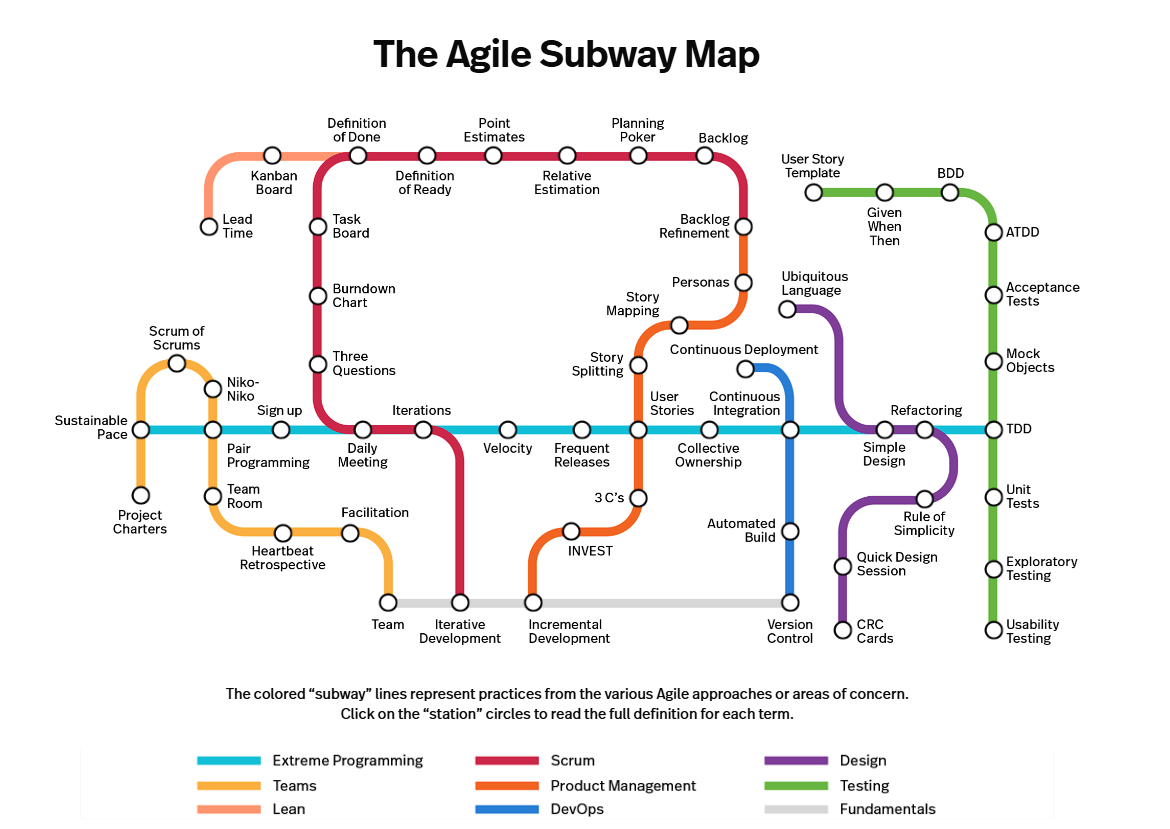
\includegraphics[width=0.8\textwidth]{img/3.1 Agile Subway Map.png}
\caption{Agile Subway Map}
\label{fig:Agile Subway Map}
\end{figure}

Estas métricas se implementan mediante un sistema de reglas automatizadas que evalúan si ciertos umbrales se cumplen o no, y que pueden ser ajustadas según el contexto (proyecto académico, industrial, etc.). Este enfoque modular permite adaptar el análisis a diferentes necesidades, manteniendo siempre un criterio objetivo y reproducible.

La aplicación analiza la actividad de un repositorio de GitHub para determinar el grado de adopción de prácticas ágiles en el desarrollo software. Para ello, se recopilan 10 reglas definidas en la ya mencionada página de \textit{Subway Map to Agile Practices}~\cite{agileSubwayMap}, y organizadas por familias (Scrum, Extreme Programming, DevOps, etc.).

Esta formalización no solo ayudan a evaluar objetivamente el proceso de desarrollo de un repositorio, sino que también proporcionan visual y detalladamente a los usuarios sugerencias claras sobre cómo mejorar su adopción de prácticas ágiles.

A continuación se detalla esta formalización, su justificación y el modo en que es evaluada mediante las 10 reglas definidas por la aplicación.

\subsection{DevOps – Automated Build}

\begin{itemize}
  \item \textbf{Descripción:} El proyecto debe incluir automatización del proceso de construcción, integración o despliegue.
  \item \textbf{Criterio de evaluación:} El asistente detecta si existen ficheros de \textit{workflows} (por ejemplo, bajo \texttt{.github/workflows}) que definan procesos automáticos usando GitHub Actions.
  \item \textbf{Importancia:} Favorece la repetibilidad, estandarización y reducción de errores humanos.
\end{itemize}

\subsection{DevOps – Version Control}

\begin{itemize}
  \item \textbf{Descripción:} Uso activo y adecuado del control de versiones.
  \item \textbf{Criterio de evaluación:} Se analiza la frecuencia de los \textit{commits}, que estos tengan título, descripción y que estén vinculados a \textit{issues} mediante \texttt{\#id} o \texttt{fixes \#id}.
  \item \textbf{Importancia:} Mejora la trazabilidad, control del código y colaboración entre miembros.
\end{itemize}

\subsection{DevOps, Extreme Programming – Continuous Integration}

\begin{itemize}
  \item \textbf{Descripción:} El repositorio debe integrar cambios frecuentemente, ejecutando pruebas automáticas.
  \item \textbf{Criterio de evaluación:} Se mide el porcentaje de éxito de los \textit{workflows} automáticos, la frecuencia de su ejecución y el uso de \textit{pull requests} para introducir cambios.
  \item \textbf{Importancia:} Detecta errores pronto y reduce conflictos al integrar código.
\end{itemize}

\subsection{Scrum – Definition of Done}

\begin{itemize}
  \item \textbf{Descripción:} Las tareas deben darse por completadas de forma inequívoca.
  \item \textbf{Criterio de evaluación:} El asistente compara el número de \textit{issues} abiertas y cerradas, asegurando que las cerradas no se vuelven a abrir.
  \item \textbf{Importancia:} Establece una línea clara sobre lo que se considera terminado y entrega de valor.
\end{itemize}

\subsection{Scrum – Backlog Quality}

\begin{itemize}
  \item \textbf{Descripción:} El backlog del proyecto debe estar compuesto por \textit{issues} claras, bien documentadas y priorizadas.
  \item \textbf{Criterio de evaluación:} Se comprueba que las \textit{issues} tengan descripción (preferiblemente con imágenes o checklists), personas asignadas y etiquetas.
  \item \textbf{Importancia:} Permite gestionar el trabajo pendiente de forma organizada.
\end{itemize}

\subsection{Scrum, Extreme Programming – Iterations}

\begin{itemize}
  \item \textbf{Descripción:} El proyecto debe avanzar por ciclos iterativos como sprints.
  \item \textbf{Criterio de evaluación:} Se analiza si se utilizan milestones, así como la frecuencia de \textit{commits}, merges y \textit{releases} por ciclo.
  \item \textbf{Importancia:} Favorece la entrega frecuente de valor y mejora continua.
\end{itemize}

\subsection{Extreme Programming – Velocity}

\begin{itemize}
  \item \textbf{Descripción:} El equipo debe ser capaz de medir su velocidad de entrega de funcionalidades.
  \item \textbf{Criterio de evaluación:} Se revisa el uso de etiquetas con story points o complejidad, así como el número de \textit{issues} cerradas por milestone o cada 15 días.
  \item \textbf{Importancia:} Permite planificar mejor la carga de trabajo y tomar decisiones basadas en datos.
\end{itemize}

\subsection{Extreme Programming – Frequent \textit{releases}}

\begin{itemize}
  \item \textbf{Descripción:} El proyecto debe generar versiones o \textit{releases} con frecuencia.
  \item \textbf{Criterio de evaluación:} Se comprueba la existencia de \textit{releases} en GitHub y la periodicidad con que se publican.
  \item \textbf{Importancia:} Permite validar funcionalidad de forma incremental y tener feedback temprano de usuarios.
\end{itemize}

\subsection{Extreme Programming – Collective Ownership}

\begin{itemize}
  \item \textbf{Descripción:} Todo miembro del equipo puede modificar cualquier parte del código.
  \item \textbf{Criterio de evaluación:} Se analiza que haya varios autores haciendo \textit{commits}, revisando \textit{pull requests}, resolviendo \textit{issues} y participando activamente en diferentes partes del repositorio.
  \item \textbf{Importancia:} Fomenta la colaboración y reduce los cuellos de botella únicos en Extreme Programming.
\end{itemize}

\subsection{Extreme Programming – Pair Programming}

\begin{itemize}
  \item \textbf{Descripción:} Los miembros colaboran en el desarrollo a través de la programación en pareja.
  \item \textbf{Criterio de evaluación:} Se detectan menciones a otros miembros en \textit{commits}, \textit{pull requests} o \textit{issues} (@usuario), así como asignaciones múltiples en tareas.
  \item \textbf{Importancia:} Mejora la calidad del código y favorece el aprendizaje mutuo.
\end{itemize}

\subsection{Resumen de prácticas evaluadas por la aplicación}
\begin{table}[H]
\centering
\small
\makebox[\textwidth]{
\begin{tabular}{l l l}
\textbf{Nombre} & \textbf{Criterio evaluado} & \textbf{Práctica Ágil asociada} \\
\hline
Automated Build & Presencia de \textit{workflows} de GitHub Actions & DevOps \\
Version Control & Frecuencia y calidad de \textit{commits} & DevOps \\
Continuous Integration & Éxito y frecuencia de \textit{workflows} y \textit{pull requests} & DevOps, XP \\
Definition of Done & \textit{issues} cerradas correctamente & Scrum \\
Backlog Quality & Calidad y estructura de \textit{issues} & Scrum \\
Iterations & Uso de milestones y ciclos de \textit{commits} & Scrum, XP \\
Velocity & Story points y métricas cada 15 días & XP \\
Frequent \textit{releases} & \textit{releases} frecuentes en el tiempo & XP \\
Collective Ownership & Participación múltiple en tareas y \textit{pull requests} & XP \\
Pair Programming & Menciones y asignaciones múltiples & XP \\
\end{tabular}
}
\caption{Resumen de reglas ágiles evaluadas por la aplicación}
\label{tab:reglasagiles}
\end{table}
